% !TeX root = RJwrapper.tex
\title{Measuring the Extent and Patterns of Urban Shrinkage for Small Towns Using R}
\author{by Cristiana Vîlcea, Liliana Popescu and Alin Clincea}

\maketitle

\abstract{Urban shrinking is a phenomenon as common as urban expansion nowadays and it affects urban settlements of all sizes, especially from developed and industrialized countries in Europe, America and Asia. The paper aims to assess the patterns of shrinkage for small and medium sized towns in Oltenia region (Romania), considering demographic, economic and social indicators with a methodological approach which considers the use of different functions and applications of R packages. Thirteen selected indicators are analysed to perform the multivariate analysis on Principal Component Analysis using the \code{prcomp()} function and the \CRANpkg{ggplot2} package to visualize the patterns of urban shrinkage. Two composite indicators were additionally created to measure the extent of urban shrinkage: CSI (Composite Shrinking Index) and RDC (Regional Demographic Change) for two-time intervals. Based on the CSI, three major categories of shrinking were observed: persistent shrinkage, mild shrinking or slow evolution toward shrinking, where the vast majority of towns are found (including mining towns, where there still is a delayed restructuring of state-owned enterprises, and towns characterised by the agrarization of local economies), and stagnant/stabilized shrinkage.}

\section{Introduction}

Shrinking cities, considered up until recently a politically taboo subject in Europe, systematically disregarded as a dominant development trend of some urban areas \citep{wiechmann_what_2007, nelle_urban_2017}, and a stigmatized topic in planning research \citep{pallagst_viewpoint_2010}, are ever more present among the research topic of various scholars throughout the world, as well as the agenda of public authorities and policy makers. Thus, the concept of shrinking cities differs from the classic notion of urban decline since new processes are at stake \citep{cunningham-sabot_theoretical_2014}.

From a historical perspective, the current period of shrinkage is distinguishable from the earlier period of decline and an earlier period of growth as well, mainly due to the prevalence of population loss, less so in its severity and not in its persistence or lack thereof \citep{beauregard_shrinking_2013}. Today, the concept of shrinking cities connotes the urban degenerative effects of the breakdown of Fordist agglomeration economies, as well as the effects of urban agglomerative and dissipative forces associated with the global diffusion of contemporary, post-Fordist systems of production \citep{audirac_shrinking_2014}.

Beginning with the 20th century, shrinking cities have developed continuously into a global phenomenon, being located mainly in Central Europe, the US, Japan and Eastern European transformation countries \citep{oswalt_atlas_2006}. They tend to have a common industrial past and are now faced with large challenges as a result of economic restructuring \citep{urban_audit_state_2007}. In Europe, the number of growing cities has been falling steadily since the 1960s, while almost a quarter (24\%) of the cities have registered a medium-term decline (almost half of all the Russian, Polish and Romanian cities with a population over 200,000 inhabitants) and more than a third showed a clear downturn since 1990 \citep{turok_trajectories_2007}. Still, the phenomenon is not equally spread throughout Europe, some countries and regions being more affected, i.e. post socialist countries, where almost half of cities can be described as shrinking \citep{wiechmann_urban_2013}, while others, such as France, experiencing a more-limited intensity in terms of number of cities affected and population loss \citep{wolff_shrinking_2013}.

Since the publication of \textit{Die Schrympfende Stadt (the Shrinking City)} \citep{gob_schrumpfende_1977} and \textit{Coping with City Shrinkage} \citep{breckenfeld_coping_1978}, some of the ways of understanding the city have changed in emphasis. Researchers’ efforts have focused on capturing the main features of the phenomenon due to its role in the reconfiguration of the urban space, which resulted in a substantial literature on urban shrinking that is undoubtedly an incontrovertible and increasingly important phenomenon, and a major challenge for future urban policies \citep{agirre-maskariano_politiques_2019, bernt_policy_2012, mallach_shrinking_2017, nelle_urban_2017, pallagst_viewpoint_2010, wiechmann_responding_2015, wiechmann_urban_2013}.

The last two decades saw an emergence of a corpus of research and projects designed to assess general causes and models of shrinkage. Several authors identify four to five major drivers for shrinkage, which are often found in a combination of two or more of these causes: i) suburbanization (flight of people and jobs to the suburbs, hollowing out of the core city, triggered by urban sprawl)\citep{wiechmann_types_2006, wiechmann_responding_2015, cunningham-sabot_theoretical_2014, audirac_shrinking_2014, reckien_why_2011, wiechmann_responding_2015}, ii) economic decline and industrial transformation \citep{wiechmann_types_2006, rink_addressing_2010, haase_conceptualizing_2014}, iii) demographic change (e.g. falling birth rates, outmigration in rural depopulation areas) \citep{rink_addressing_2010, haase_conceptualizing_2014, wiechmann_responding_2015}; iv) structural upheaval (economic reorganization, collapse of an entire political system, unrest, resettlements) and environmental pollution \citep{wiechmann_types_2006, haase_conceptualizing_2014, cunningham-sabot_theoretical_2014, wiechmann_responding_2015}.

Over the past decades, shrinkage has become a "normal pathway" of development for cities and regions all across Europe \citep{rink_addressing_2010}. Recent writing and research on the shrinking cities have also focused on indicators of urban shrinkage, which should be necessarily dynamic and capable of detecting medium-term tendencies, distinguishing between episodic or acute shrinkage (when developments fluctuate in a certain period, but have an overall negative evaluation) and continuous or chronic shrinking \citep{wolff_indicators_2014}. Since population loss, which is an initial clue of urban processes and a major indicator for urban shrinkage, does not encompass the various aspects of the phenomenon, there is a continuous focus on indicators to measure shrinking cities. They can be summarized into three main categories: demographic indicators, economic indicators and social indicators.

Among the demographic indicators, migration, population natural increase and a shifting population structure (ageing and feminization) are key factors of population decline, highly connected to other social, economic and built environment variables \citep{turok_trajectories_2007, guimaraes_shrinking_2015, haase_varieties_2016, banica_challenges_2017, cauchi-duval_decroissance_2017, hartt_how_2018}. Indicators related to economic changes (employment, unemployment, firms, services) are more difficult to gather and raise issues in terms of comparability among countries \citep{martinez-fernandez_shrinking_2015}, but should not be neglected as the economic decline is among the drivers of shrinkage. Social indicators usually considered when analysing shrinkage refer either to households (housing permit rates, housing start rate, number of households) \citep{bontje_facing_2004, wolff_indicators_2014, guimaraes_shrinking_2015, lauf_effects_2016, hartt_how_2018}, or to the number of students enrolled in education units \citep{guimaraes_shrinking_2015}. This decreases attractiveness of a city as an educational place. Consequently, it causes a decreasing number of students enrolled in compulsory education levels and the closure of educational institutions \citep{wolff_indicators_2014}.

Most of the studies regarding shrinking cities focus on larger urban centres, exceeding two hundred thousand inhabitants. However, many of the spatial planning and development strategies of the European Union focus on small and medium-sized towns, often seen as the chronic patients of regional policy, constantly in need of care but never getting well \citep{wirth_peripheralisation_2016}. Most of the French shrinking cities are small urban areas, with less than 50,000 inhabitants, while in Germany the most dramatic decrease occurs in medium sized cities \citep{martinez-fernandez_shrinking_2015}. In Hungary, almost every small town has shrunk during at least the last decade \citep{pirisi_between_2015}. In Romania, the discussion within urban planning has also begun, despite focusing on some larger towns, researchers from various fields drawing attention to this issue \citep{banica_challenges_2017, jucu_economic_2016, jucu_post-communist_2019, paun_constantinescu_shrinking_2019, popescu_deindustrialization_2014, schoenberg_urban_2014, stoica_exploring_2020, steinfuhrer_small_2020} since the Romanian towns clearly witness a decline on short or medium term, which is uneven, but in perpetuum \citep{paun_constantinescu_shrinking_2013}.

\section{Data and methods}

The multidimensional concept of shrinking cities has a comprehensive meaning, as the drivers which determine this process are complex (demographic, economic, social). Therefore official statistics from the last three censuses (1992, 2002, 2011) and from 2018 were used to calculate indicators. We applied simple standard formulae in population geography regarding the demographic and economic phenomena such as population natural increase, feminization, migration, ageing, unemployment, i.e. \textit{k}\textsubscript{1}-\textit{k}\textsubscript{6} and construct composite indices. All indices used in the analysis of this phenomenon were based on their importance and relationship to each other and to the concept itself. After a thorough documentation focusing on other studies referring to shrinking cities \citep{haase_varieties_2016, hartt_how_2018, mallach_shrinking_2017, rink_addressing_2010, wiechmann_responding_2015, wiechmann_urban_2013} we selected a series of demographic and socio-economic indicators that met the criteria of availability and relevance for the study. Availability and consistency of data for small Romanian towns represented a major issue, as there are missing time series and uneven statistics. Thus, in order to perform the calculation without errors caused by missing values, authors imputed these missing values with zero, as the frequency of missingness was not high and it was observed that zero imputing does not affect the results of the study. This major issue played an important role in the selection of the best indicators considered for the multivariate analysis and the aggregation method. The chosen indicators vary in terms of measurement unit, as they are expressed as absolute or computed data (Table \ref{table:1}), but we also weighted their strengths and weaknesses.

\begin{table}[ht]
	\centering
	\small
	\begin{tabular}{ ccc }
		\toprule
		\textbf{Selected indices}                               & \textbf{M.U.}             & \textbf{Assigned code} \\
		\midrule
		\multicolumn{3}{l}{\textbf{Demographic indicators}}                                      \\
		\midrule
		\multicolumn{1}{l}{migration rate}           & \textperthousand & $k_1$         \\
		\multicolumn{1}{l}{rate of natural increase} & \textperthousand & $k_2$         \\
		\multicolumn{1}{l}{feminization index}       & \%               & $k_3$         \\
		\multicolumn{1}{l}{elderly population}       & \%               & $k_4$         \\
		\multicolumn{1}{l}{mean age}                 & \%               & $k_5$         \\
		\midrule
		\multicolumn{3}{l}{\textbf{Economic indicators}}                                         \\
		\midrule
		\multicolumn{1}{l}{unemployment rate}        & \%               & $k_6$         \\
		\multicolumn{1}{l}{employees}                & number           & $k_7$         \\
		\midrule
		\multicolumn{3}{l}{\textbf{Social indicators}}                                           \\
		\midrule
		\multicolumn{1}{l}{households}               & number           & $k_8$         \\
		\multicolumn{1}{l}{libraries}                & number           & $k_9$         \\
		\multicolumn{1}{l}{doctors}                  & number           & $k_{10}$      \\
		\multicolumn{1}{l}{students}                 & number           & $k_{11}$      \\
		\multicolumn{1}{l}{education}                & number           & $k_{12}$      \\
		\multicolumn{1}{l}{hospital beds}            & number           & $k_{13}$      \\
		\bottomrule
	\end{tabular}
	\caption{The selection of indicators used for aggregation.}
	\label{table:1}
\end{table}

The work flow consists in several stages, the main step concentrating on the creation and use of the composite indicators (CSI and RDC) (Figure \ref{figure:workflow}).

\begin{figure}[!htbp]
	\centering
	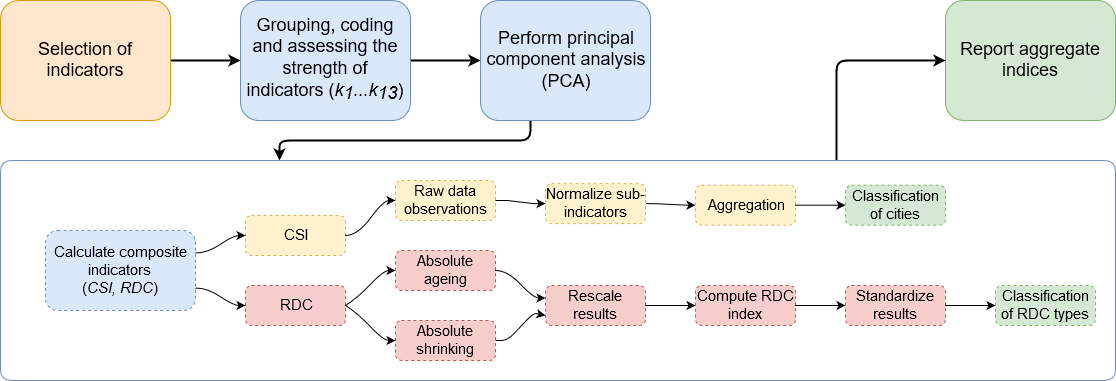
\includegraphics[width=1\textwidth]{workflow}
	\caption{Overall workflow for the research methodology, depicting the main steps of the process, from the selection of indicators to the resulting aggregate indices.}
	\label{figure:workflow}
\end{figure}

As defined by \citet{oecd_handbook_2008} in the Glossary of Statistical terms \textit{"a composite indicator is obtained from the combination of individual indicators into a single index, on the basis of an underlying model of the multidimensional concept that is being measured"}.

The study uses two types of composite indices to observe and analyse the dynamics of the shrinking process specific for the cities in the South West Development Region of Oltenia. The first composite indicator used is the Regional Demographic Change (RDC) obtained by applying the methodology described by \citet{tivig_mapping_2008} in the \textit{Final Report of the Mapping Regional Demographic Change and Regional Demographic Location Risk in Europe}. The RDC index was initially used to describe the process of ageing and shrinking of the population in 27 European states from 264 regions. We adapted the methodology to compute this index for 34 towns located in the South West Development Region of Oltenia. The RDC index captures the extent and time-path of demographic change by accounting for two of its dimensions: population ageing with the perspective of shrinking. The RDC index is calculated using raw indicators for age, like the mean age, and population size like population density. Based on these two indicators for population age and density, the ageing and shrinking process are calculated and assessed in absolute terms for each town and three periods of time (please see research data, sheet \textit{mean\_age} and \textit{density} for calculated data). Thus, the index was calculated for 3 time-intervals: 1992-2018; 2018-2030 and 1992-2030. In order to be able to make cross-period comparison, a rescaling was necessary. For analyzing the relative position of the towns within the region in terms of ageing and shrinking the values computed previously had been z-standardized \citep{tivig_mapping_2008}. If the RDC index shows the demographic change that takes place in the small towns under analysis, the RDC type indicate whether their population ages faster or slower and grows less or shrinks as compared to the average of the region. The four types of the RDC-index were applied to one regional dimension (South West Development Region of Oltenia) and represented showing the overall trend (1992-2030) and the future trend (2018-2030).

The second composite indicator (CSI) was created based on thirteen sub-indices (\textit{k}\textsubscript{1}\dots\textsubscript{13}) computed for all 34 towns located in the study area and aggregated into a single index using the additive method \citep{gan_when_2017, nardo_tools_2005, oecd_handbook_2008, saisana_state_2002, syrovatka_measuring_2019}. The additive aggregation method, and especially the weighted arithmetic mean, is the widest used method \citep{gan_when_2017, pollesch_applications_2015} as it sums up the normalized values of sub-indicators.
The Principal Component Analysis (PCA) was performed to analyse the correlation between the sub-indicators. We intended to use similar indicators as in other studies (Table \ref{table:1}), but approach a different method and process data in R. The multiple packages make this language a powerful tool for data processing and visualization \citep{barry_collections_2018} with multiple possibilities of application, especially in spatial analysis \citep{lovelace_geocomputation_2019}. As the sub-indicators had different measurement scales, variable standardization was handled using the option \code{scale=true} in \code{prcomp()}. Complying with the minimum required rule of 3:1 \citep{jollands_usefulness_2003}, the use of this method allows summarizing the entire set of individual indicators \citep{paul_methodological_2013, jolliffe_principal_2016}, while preserving the maximum possible proportion of the total variation in the original data set \citep{sharma_applied_1996}. The PCA results were represented using the \pkg{ggplot2} package \citep{kassambara_r_2017, wickham_ggplot2_2016}.

\section{Results}

PCA was used to analyse the interrelationships among all thirteen variables (Table \ref{table:1}) observed in 34 small towns located in Oltenia region, in two reference years 1992 and 2018. The main characteristic of this method is the reduction of a great number of variables to a smaller number (principal components), as linear combinations of the variables in the multivariate set, with minimum loss of information. Principal components outputs where computed using \code{prcomp()} for an improved numerical accuracy and displayed using \code{screeplot()}.

\begin{figure}[htbp]
	\centering
	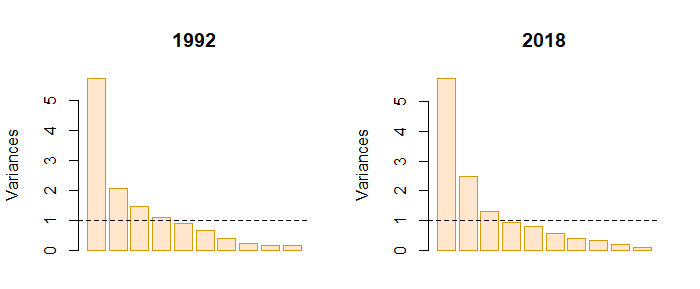
\includegraphics[width=1\textwidth]{screeplot}
	\caption{Scree plot of the principal components. The graphic representation of variances allows for easier selection of relevant components.}
	\label{figure:screeplot}
\end{figure}

Analysing the scree plots, there are small differences in the eigenvalues of the components comparing the two years observed (Figure \ref{figure:screeplot}). If we use the Kaiser criterion, we see that only the first four (1992), respectively three (2018) components have eigenvalues greater than 1. But these components explain only 79.5\% of the variation in the data for 1992 and 73.2\% for 2018 and usually a cumulative proportion of at least 85\%, that explain an acceptable level of variance, is obtained by the first five principal components. The fourth and fifth eigenvalues of the principal components in 2018 are only close to the value of 1. Therefore, values which are greater than 0.75 are considered as "strong". For an acceptable level of variance, we selected the first five principal components for analysis (Table \ref{table:2}).

\begin{table}[!ht]
	\centering
	\fontsize{5.7}{6.6} \selectfont
	\begin{tabular}{ cccccccccccccc }
		\toprule
		1992                             & {\color{orange}\textbf{PC(1)}}  & {\color{orange}\textbf{PC(2)}}  & {\color{orange}\textbf{PC(3)}}  & PC(4)  & PC(5)  & PC(6)  & PC(7)  & PC(8)  & PC(9)  & PC(10) & PC(11) & PC(12) & PC(13)  \\
		\midrule
		\multicolumn{1}{l}{Std. dev.}  & 2.40   & 1.48   & 1.16   & 1.04   & 0.95   & 0.83   & 0.63   & 0.47   & 0.40   & 0.37   & 0.29   & 0.21   & 0.15    \\
		\multicolumn{1}{l}{Variance}   & 0.44   & 0.17   & 0.10   & 0.08   & 0.07   & 0.05   & 0.03   & 0.02   & 0.01   & 0.01   & 0.01   & 0.00   & 0.00    \\
		\multicolumn{1}{l}{Cumulative} & 44.2\% & 61.0\% & 71.3\% & 79.5\% & 86.5\% & 91.7\% & 94.8\% & 96.5\% & 97.8\% & 98.8\% & 99.5\% & 99.8\% & 100.0\% \\

		\bottomrule
		\toprule
		2018                             & {\color{orange}\textbf{PC(1)}}  & {\color{orange}\textbf{PC(2)}}  & {\color{orange}\textbf{PC(3)}} & PC(4)  & PC(5)  & PC(6)  & PC(7)  & PC(8)  & PC(9)  & PC(10) & PC(11) & PC(12) & PC(13)  \\
		\midrule
		\multicolumn{1}{l}{Std. dev.}  & 2.39   & 1.57   & 1.16   & 0.97   & 0.92   & 0.75   & 0.62   & 0.56   & 0.45   & 0.30   & 0.27   & 0.21   & 0.18    \\
		\multicolumn{1}{l}{Variance}   & 0.44   & 0.19   & 0.10   & 0.07   & 0.07   & 0.04   & 0.03   & 0.02   & 0.02   & 0.01   & 0.01   & 0.00   & 0.00    \\
		\multicolumn{1}{l}{Cumulative} & 44.0\% & 62.9\% & 73.2\% & 80.4\% & 86.9\% & 91.3\% & 94.3\% & 96.6\% & 98.2\% & 98.8\% & 99.4\% & 99.7\% & 100.0\% \\
		\bottomrule
	\end{tabular}
	\caption{Summary of Principal Component Analysis (PCA) used for the selection of principal components. The  components with a cumulative variance above 0.75 are considered "strong".}
	\label{table:2}
\end{table}

Preliminary data analysis indicates a small difference in variance and proportion for the first five components, in the two reference years (Table \ref{table:3}). The data showed that the highest value of the variable is 0.690, respectively 0.634 (Table \ref{table:4}), therefore we considered that the level of correlation between each component is important above the value of 0.3.

\begin{table}[!htb]
	\centering
	\small
	\begin{tabular}{ lccccc }
		\toprule
		\text{} & PC1     & PC2    & PC3    & PC4    & PC5    \\
		\midrule
		1992    & 44.2\%  & 61.0\% & 71.3\% & 79.5\% & 86.5\% \\
		2018    & 44.0\%  & 62.9\% & 73.2\% & 80.4\% & 86.9\% \\
		\midrule
		change  & -0.0018 & 0.0188 & 0.0190 & 0.0083 & 0.0042 \\
		\bottomrule
	\end{tabular}
	\caption{Changes in the variances of the first five principal components in the analyzed time interval: 1992-2018.}
	\label{table:3}
\end{table}

\begin{table}[htb]
	\centering
	\fontsize{8.5}{10.2} \selectfont
	\begin{tabular}{ lrrrrr|rrrrr }
		\toprule
		\multicolumn{1}{c}{}  & \multicolumn{5}{c|}{Principal Component (1992)} & \multicolumn{5}{c}{Principal Component (2018)}                                                                                                                                                                                 \\
		\midrule
		Variable & PC(1)                                             & PC(2)                                            & PC(3)               & PC(4)               & PC(5)               & PC(1)               & PC(2)               & PC(3)               & PC(4)               & PC(5)               \\
		\midrule
		$k_{1}$  & 0.076                                             & -0.338                                           & \color{red}{-0.644} & 0.064               & \color{red}{-0.419} & 0.407               & -0.035              & \color{red}{-0.648} & \color{red}{-0.476} & -0.023              \\
		$k_{2}$  & 0.000                                             & \color{red}{-0.588}                              & -0.175              & \color{red}{-0.713} & -0.042              & 0.128               & \color{red}{-0.613} & -0.013              & \color{red}{-0.614} & -0.084              \\
		$k_{3}$  & -0.350                                            & \color{red}{0.642}                               & -0.129              & \color{red}{-0.522} & 0.278               & -0.621              & \color{red}{0.600}  & -0.153              & -0.015              & 0.133               \\
		$k_{4}$  & -0.711                                            & \color{red}{0.557}                               & 0.089               & -0.113              & -0.240              & 0.338               & \color{red}{0.843}  & -0.279              & -0.047              & -0.158              \\
		$k_{5}$  & -0.483                                            & \color{red}{0.636}                               & 0.215               & 0.128               & -0.130              & 0.043               & \color{red}{0.893}  & 0.164               & -0.154              & -0.010              \\
		$k_{6}$  & 0.233                                             & \color{red}{0.487}                               & \color{red}{-0.708} & 0.142               & -0.096              & 0.094               & -0.384              & \color{red}{-0.671} & \color{red}{0.528}  & -0.060              \\
		$k_{7}$  & \color{red}{0.903}                                & -0.175                                           & 0.223               & 0.170               & 0.125               & \color{red}{-0.757} & -0.215              & \color{red}{0.397}  & -0.021              & 0.186               \\
		$k_{8}$  & \color{red}{0.935}                                & 0.212                                            & 0.051               & 0.064               & -0.022              & \color{red}{-0.936} & -0.031              & 0.045               & 0.001               & -0.210              \\
		$k_{9}$  & 0.683                                             & 0.266                                            & 0.145               & -0.056              & \color{red}{-0.546} & \color{red}{-0.832} & 0.071               & -0.183              & -0.095              & \color{red}{-0.342} \\
		$k_{10}$ & \color{red}{0.806}                                & 0.355                                            & -0.322              & -0.054              & 0.186               & \color{red}{-0.841} & 0.045               & -0.286              & -0.037              & \color{red}{0.366}  \\
		$k_{11}$ & \color{red}{0.947}                                & 0.020                                            & 0.148               & 0.015               & 0.005               & \color{red}{-0.900} & -0.067              & -0.083              & -0.005              & -0.211              \\
		$k_{12}$ & 0.697                                             & 0.175                                            & 0.313               & \color{red}{-0.433} & \color{red}{-0.323} & \color{red}{-0.871} & -0.030              & -0.011              & -0.018              & \color{red}{-0.395} \\
		$k_{13}$ & \color{red}{0.798}                                & 0.239                                            & -0.140              & -0.104              & \color{red}{0.337}  & \color{red}{-0.783} & 0.004               & -0.238              & -0.116              & \color{red}{0.517}  \\
		\bottomrule
	\end{tabular}
	\caption{The first five values of the principal components for the variables $k_{1}$-$k_{13}$ in 1992 and 2018.}
	\label{table:4}
\end{table}

For this set of results, the first principal component is strongly correlated with almost all the original variables of the social and economic factors in 1992 and 2018. It has exclusively negative correlations with almost all (except unemployment rate) variables observed in 2018. So, this component measures primarily the social-economic factors that influence the shrinking process of small cities. The second component measures the demographic dimension of shirking, as it has negative correlations for the rate of natural increase and positive correlations for the rest of the demographic variables like the feminization index, the percent of elders and the mean age. This fact suggests that the five criteria in 1992 and six in 2018 vary together, increasing or decreasing. The third and fourth components indicate correlations with both economic and demographic variables. The third component has negative correlations in 1992 and positive in 2018 for the migration rate and unemployment rate. In 2018, the third component is also strongly correlated with the number of employees. The fourth component shows a shift in correlations, as they are positive in 1992 with the introduction of a variable from the social sector (number of schools) and negative in 2018 for the demographic variables, but positive for the unemployment rate. The fifth component indicates also several changes in 2018 as compared to 1992, because in 2018 it has correlations only for the social variables (positive for the number of doctors and hospital beds and negative correlations for the number of libraries and schools) (Table \ref{table:4}).

The scope of this analysis is to identify the directions (principal components) along which the variation in the data is the highest. As the first two components account for most of the variance in the date, to achieve this goal, the dimensionality of the multivariate data was reduced into two principal components, in order to be able to visualize them graphically. The two graphs were generated in R using the \pkg{ggplot2}, \CRANpkg{ggrepel}, \CRANpkg{gridExtra} and \CRANpkg{readxl} packages (see \code{shrinking\_cities.r} from supplemental material).

The graphic visualization of the results allows to analyse the variance of the variables and the change in direction trends for 1992 and 2018. Analysing the scores of the second principal component versus the scores of the first principal component, we notice that, in 1992, the first principal component has large positive associations with the number of houses, libraries, doctors, pupils, schools and hospital beds and negative associations with the number of employees. So, it measures mainly the social dimension of the cities as shrinkage factors. The second component measures primarily the demographic dimension as it has large positive loadings on the rate of elders and mean age (Figure \ref{figure:pca}, 1992). This aspect is changing entirely in 2018, if we observe the directions along which we have the highest variance of the date. Thus, the demographic variables (migration rate and elders) strongly influence component 1, while the social-economic variables influence the second component. For a better view of differences amongst towns, the points representing the urban settlements, vary in size and intensity according to the values of the third and fourth components (Figure \ref{figure:pca}, 2018).

\begin{figure}[htbp]
	\centering
	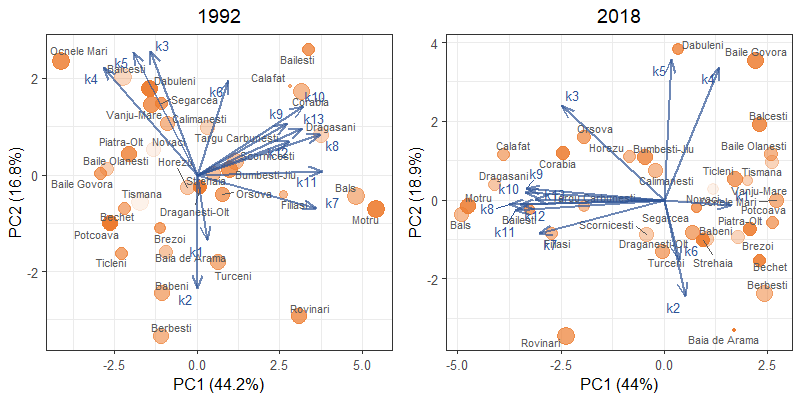
\includegraphics[width=1\textwidth]{pca}
	\caption{Principal Components Analysis of shrinkage indicators}
	\label{figure:pca}
\end{figure}

The changes in population, especially the processes of ageing and shrinking, have a direct influence on the socio-economic dimension of settlements. As in most European countries, the ageing of the population is a phenomenon that characterizes almost all the settlements in Romania and will continue, but with different intensities; however, ageing greatly varies among the towns considered for analysis. The dimension of shrinking is given by the decrease in the number of inhabitants, which is better expressed by the decrease in the population density. The data indicated that, same as the ageing process, depopulation is another characteristic of the selected towns.

We used the RDC index to compare, at regional level, the dimension of ageing and shrinking of all 34 small towns located in Oltenia. Three time-intervals were considered (1992-2018 - past; 2018-2030 - future and 1992-2030 - overall) to show the overall and the future trend (Figure \ref{figure:rdc}).

\begin{figure}[htbp]
	\centering
	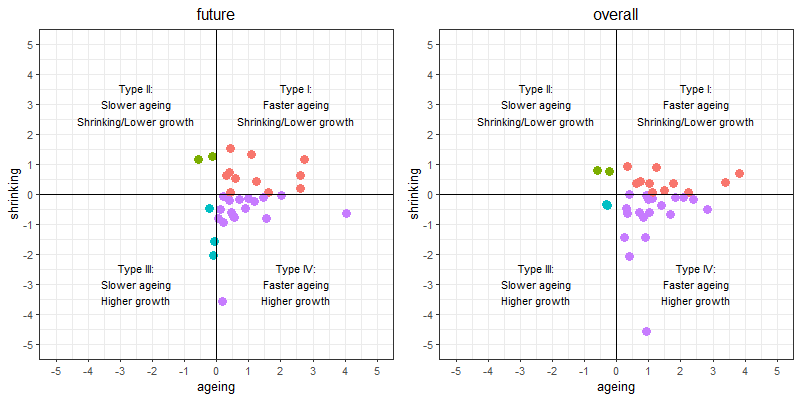
\includegraphics[width=1\textwidth]{rdc}
	\caption{Future (2018-2030, left) and Overall (1992-2030, right) trends of Regional Demographic Change (RDC-type) for small towns in South-West Development Region of Oltenia}
	\label{figure:rdc}
\end{figure}

After examining the population trend for every town, we identified four categories, differentiated by ageing, population evolution and shrinking. This shows that some towns are more resilient to shrinkage than others, due to a combination of factors. However, there is clear evidence that a significant number of towns (about 40\%) are shrinking, while 80\% face a fast-ageing process of the population.

The results indicated that there are some demographic changes between the future trend and the overall trend. If the share of towns included in the first two categories remains unchanged during the two analysed periods, their number shows a slight change for the fourth and third types. These results indicate that some settlements will pass in the future from higher growth and slower ageing (type III) to higher growth and faster ageing (IV) (Figure \ref{figure:rdc} \& Table \ref{table:5}).

\begin{table}[ht]
	\centering
	\small
	\begin{tabular}{ rlrrrr }
		\toprule
		\multicolumn{1}{c}{RDC type} & \multicolumn{1}{c}{Description} & \multicolumn{2}{c}{\makecell[c]{Future trend\\2018-2030}} & \multicolumn{2}{c}{\makecell[c]{Overall trend\\1992-2030}}\\
		\midrule
		I & Faster ageing. Shrinking/Lower growth  & 11 towns & 32\%        & 11 towns & 32\% \\
		II & Slower ageing. Shrinking/Lower growth & 2 towns & 6\%          & 2 towns & 6\%   \\
		III & Slower ageing. Higher growth         & 4 towns & 12\%         & 2 towns & 6\%   \\
		IV & Faster ageing. Higher growth          & 17 towns & 50\%        & 19 towns & 56\% \\
		\bottomrule
	\end{tabular}
	\caption{Percent of towns according to the four types of RDC}
	\label{table:5}
\end{table}

Using the composite indicator (CSI) we computed the values for the beginning and present period and analysed the dimension of change for all 34 towns at demographic and social-economic levels for the future period (2030). The indicator includes all thirteen sub-indices (Table \ref{table:1}) considered important in the shrinking process of cities. The values of CSI for 1992 and 2018 were calculated using the following formula:

\begin{equation}
	\label{formula}
	CSI = \sum_{i=1}^{n}\frac{k_{i}-min\left(k_{i}\right)}{n\left(max\left(k_{i}\right)-min\left(k_{i}\right)\right)}
\end{equation}

where:\\
\hspace*{3em}
\begin{tabular}{ll}
	$n$:                       & subindicator count            \\
	$k\textsubscript{i}$:      & selected subindicator         \\
	$min\left(k\textsubscript{i}\right)$: & minimum value of subindicator \\
	$max\left(k\textsubscript{i}\right)$: & maximum value of subindicator
\end{tabular}

To observe the shrinking trend of small towns for future period, the values for year 2030 were calculated based on the computed values of CSI for 1992, 2002, 2011 and 2018 using the forecast function in Microsoft Office Excel to predict the values for 2030. Standard deviation (St.dev.) values were calculated to observe highest values. The results were compared and represented, observing that thirteen towns have high variations and St.dev. values > 0.04 (Table \ref{table:6} \& Figure \ref{figure:scatterplot}).

\begin{table}[ht]
	\centering
	\footnotesize
	\begin{tabular}{ lcccc|lcccc }
		\toprule
		\multicolumn{1}{c}{Towns} & 1992  & 2018  & 2030  & St.dev. & \multicolumn{1}{c}{Towns} & 1992  & 2018  & 2030  & St.dev. \\
		\midrule
		Băilești                    & 0.599 & 0.554 & 0.529 & 0.036   & Vânju-Mare                  & 0.298 & 0.318 & 0.307 & 0.010   \\
		Bechet                      & 0.235 & 0.189 & 0.202 & 0.023   & Balș                        & 0.551 & 0.593 & 0.629 & 0.039   \\
		Calafat                     & 0.623 & 0.568 & 0.514 & 0.055   & Corabia                     & 0.555 & 0.486 & 0.482 & 0.041   \\
		Dăbuleni                    & 0.297 & 0.400 & 0.446 & 0.076   & Drăgănești-Olt              & 0.306 & 0.301 & 0.327 & 0.014   \\
		Filiași                     & 0.559 & 0.491 & 0.431 & 0.064   & Piatra-Olt                  & 0.245 & 0.247 & 0.249 & 0.002   \\
		Segarcea                    & 0.347 & 0.339 & 0.340 & 0.004   & Potcoava                    & 0.157 & 0.248 & 0.294 & 0.070   \\
		Tismana                     & 0.342 & 0.291 & 0.238 & 0.052   & Scornicești                 & 0.418 & 0.365 & 0.410 & 0.028   \\
		Turceni                     & 0.349 & 0.329 & 0.374 & 0.022   & Băbeni                      & 0.269 & 0.291 & 0.374 & 0.055   \\
		Bumbești-Jiu                & 0.373 & 0.326 & 0.338 & 0.025   & Băile Govora                & 0.255 & 0.232 & 0.237 & 0.012   \\
		Novaci                      & 0.393 & 0.414 & 0.422 & 0.015   & Băile Olănești              & 0.277 & 0.245 & 0.263 & 0.016   \\
		Țicleni                     & 0.259 & 0.225 & 0.220 & 0.021   & Bălcești                    & 0.350 & 0.236 & 0.214 & 0.073   \\
		Târgu Cărbunești            & 0.419 & 0.458 & 0.539 & 0.061   & Berbești                    & 0.196 & 0.196 & 0.222 & 0.015   \\
		Motru                       & 0.495 & 0.531 & 0.572 & 0.039   & Brezoi                      & 0.296 & 0.281 & 0.302 & 0.011   \\
		Rovinari                    & 0.356 & 0.365 & 0.427 & 0.038   & Călimănești                 & 0.321 & 0.385 & 0.447 & 0.063   \\
		Baia de Aramă               & 0.290 & 0.323 & 0.335 & 0.024   & Drăgășani                   & 0.572 & 0.630 & 0.709 & 0.069   \\
		Orșova                      & 0.337 & 0.476 & 0.547 & 0.107   & Horezu                      & 0.341 & 0.441 & 0.485 & 0.074   \\
		Strehaia                    & 0.361 & 0.267 & 0.236 & 0.065   & Ocnele Mari                 & 0.231 & 0.200 & 0.190 & 0.021   \\
		\bottomrule
	\end{tabular}
	\caption{The computed values of CSI for each town, showing shrinkage in 1992, 2018 and the 2030 forecast.}
	\label{table:6}
\end{table}

\begin{figure}[htbp]
	\centering
	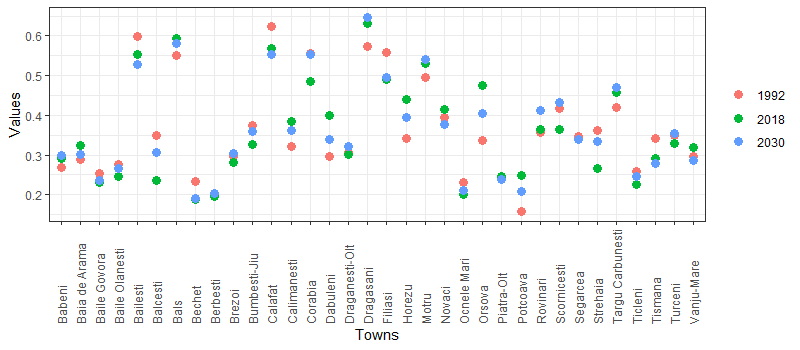
\includegraphics[width=1\textwidth]{scatterplot}
	\caption{Variation of CSI values for the reference period}
	\label{figure:scatterplot}
\end{figure}

\section{Discussions}

As we initially calculated the RDC index for all 34 towns to analyse the dimension of shrinking, we deem necessary to use a more complex index to include economic and social dimensions. \citet{tivig_mapping_2008} analyses the dimension of shrinking using only demographic indices, classifying cities in four categories. However, the scientific literature considers the topic of shrinking cities as a more complex process, which involves social and economic factors \citep{bernt_policy_2012, martinez-fernandez_shrinking_2015, wolff_indicators_2014}.

Besides the general factors, local features also contribute to the shrinking process of cities, especially for smaller ones. Therefore, we deem necessary to also use another, more complex, composite indicator. After comparing the results, we concluded that only six towns undergo a clear shrinking process, falling into the category of persistent shrinkage, while eighteen have a moderate or slow evolution toward shrinking (recent or mild shrinkage). There are also ten settlements that had a linear, almost stagnant, evolution for the entire reference period with the same future trend (Figure \ref{figure:shrinking}).

\begin{figure}[htbp]
	\centering
	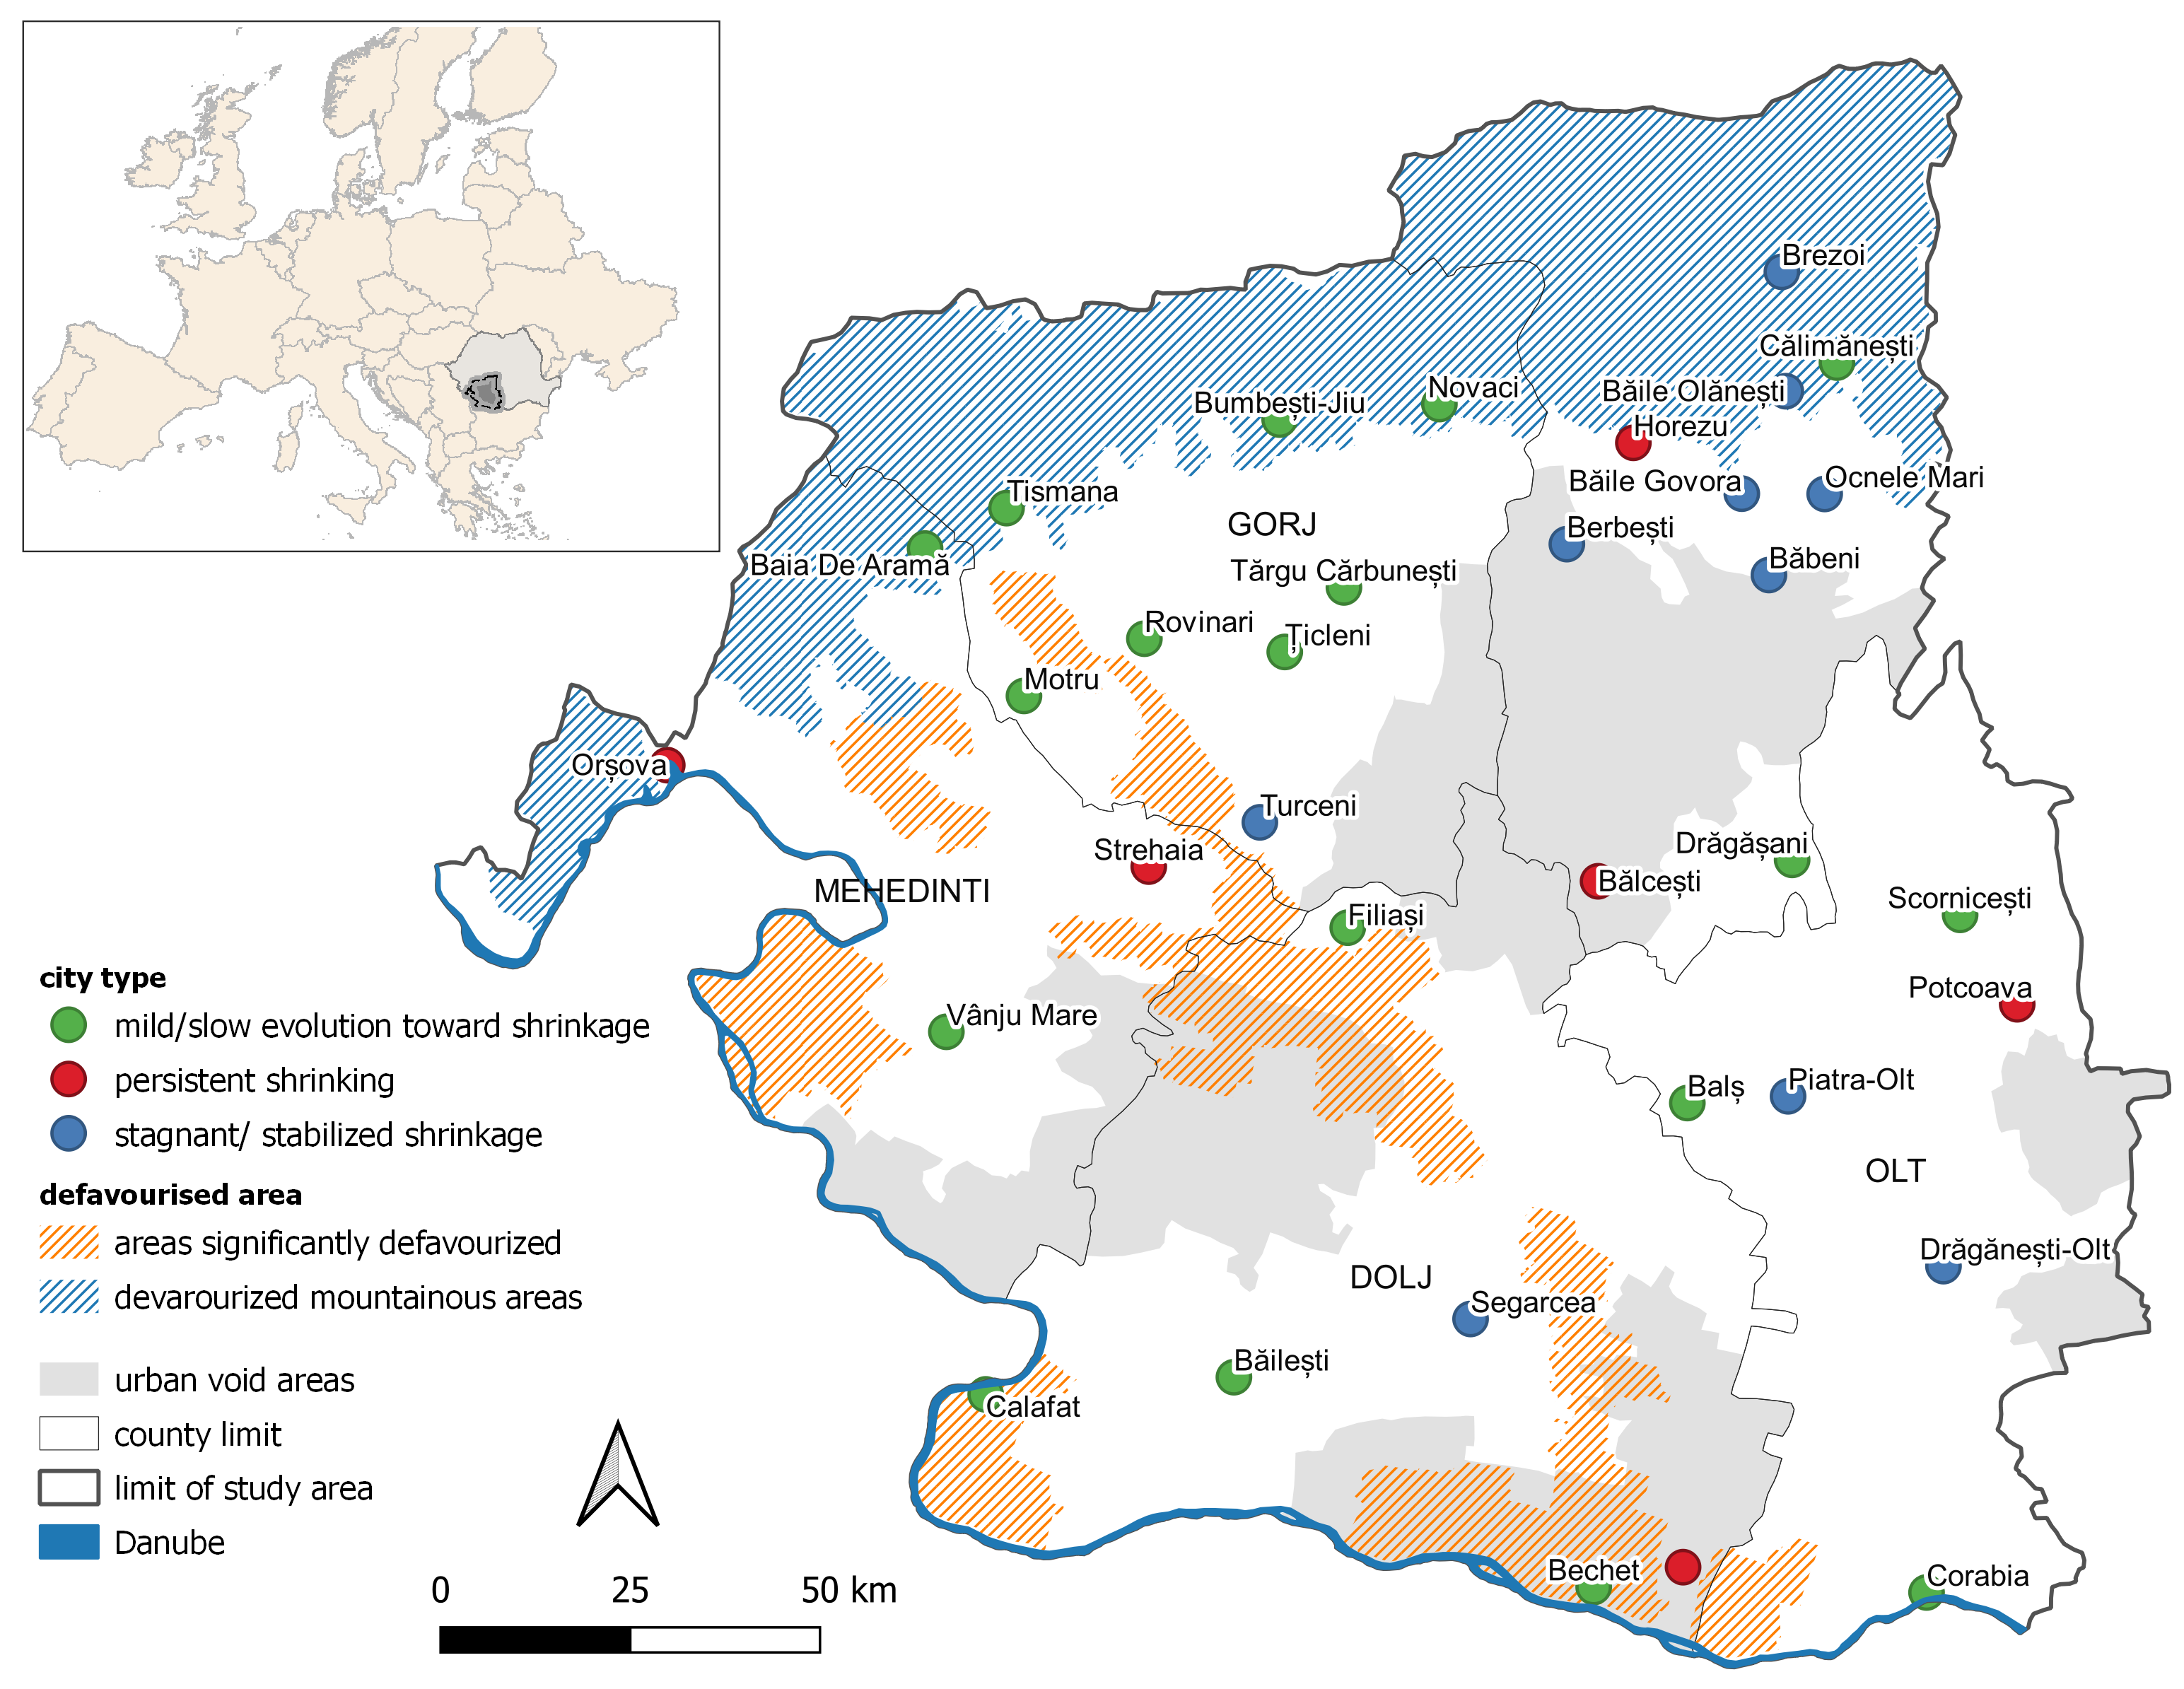
\includegraphics[width=0.9\textwidth]{shrinking}
	\caption{City types according to CSI}
	\label{figure:shrinking}
\end{figure}

According to CSI values the towns can be classified in three categories: persistent shrinkage, a mild evolution towards shrinkage and stagnant shrinkage. The first category includes only 6 towns, which is less than a fifth of the analysed towns, and except for Orșova, they did not benefit during the communist period from any state-owned flagship companies and did not have any significant industrial base. This category varies largely in terms of population size, population loss, economic activities and rural/urban characteristics. The smaller and more rural in character the town, the greater the pressure on shrinkage is. Just as in other regions, the regional and local economic restructuring alter the urban communities \citep{jucu_economic_2016}.

A mild/slow evolution toward shrinkage characterizes the towns of Băilești, Bechet, Calafat, Tismana, Bumbești, Novaci, Țicleni, Târgu Cărbunești, Filiași, Motru, Rovinari, Baia de Aramă, Vânju Mare, Balș, Corabia, Scornicești, Călimănești and Drăgășani. There is a diversity of different town types (resourced-based mining towns, old ports, rural small towns, some tourism activities), scattered throughout the entire region, testifying that there are multiple factors causing shrinkage. Few of these towns have managed to keep their industrial activities due to the strategic importance of their power plants for the production of electricity. Most of them did not succeed to foster any new economic activities, nor modernise traditional branches, so there were no major new investments since the 1980s. This situation may be partially attributed to the towns location and poor accessibility, but also lack of entrepreneurial culture and poor administration that was hardly able to cope with the economic decline and transition to the market economy.

A stagnant/stabilized shrinkage was noted for ten towns (Figure \ref{figure:shrinking}). Some of these towns have kept and developed some forms of tourism activities (holiday homes, private camps, accommodation and leisure facilities), benefiting from considerable investments following various programmes financed by the EU for fostering the tourism sector.

Small towns that relied heavily on agriculture, forestry or mining activities will continue to be affected by shrinking, which will definitely put a stain on their physical and social structure, the need for viable alternatives to smart shrinkage being of utmost importance.

This analysis provides empirical confirmation that many small towns in Oltenia are in fact shrinking, despite different economic and demographic background, and that mainly the demographic indicators (population decrease, out-migration and ageing), followed by economic ones, are the most important factors for urban shrinkage in the region. However, these towns do not only face loses of population, but also a mismatch between the physical urban structure and the population needs.

What are the main causes for shrinking in the case of small and medium towns in Oltenia? After analysing the situation in other European countries, we can definitely say that the experience of this region has some specifics, as the urban shrinkage is not caused by suburbanization and to a larger extent, neither by deindustrialization. In 1992, most (3/4) of the small and medium-small towns in the region had a location quotient of industry below the urban average of 1.029 \citep{popescu_deindustrialization_2014}, which might in part explain this situation. Moreover, these towns were ranked much lower in the urban hierarchy and had limited economic options, hosting mainly local resource-based industries.

Shrinking is rather caused by the overlapping of simultaneous demographic processes - out-migration, drops in birth rates, ageing (which leads to population decline) and economic difficulties (loss of jobs, lack of private companies, lack of entrepreneurial culture, heavy reliance on agriculture and subsidies from the government).

The current study provides a critical analysis on the extent of shrinking phenomenon that severely affects more than a third of the small and medium-size towns in the region of Oltenia and the outcomes of the post-socialist urban changes. In the long run, this shrinkage will definitely affect labour and the social and technical infrastructure, putting a great strain on the local budgets.

\section{Conclusions}

During the last decade, the issue of \textit{shrinking cities} is pervasive for the research interest of academics and the political discourse of many countries. Unfortunately, despite the evident urban decline of small Romanian towns, from both the economic and demographic perspective during the last 3 decades, the politicians and authorities seem to miss the extent of this phenomenon, which has become rather common in Romania and Oltenia region as well.

The decrease in size of the population, the increase of the mean age and the ageing of the population has repercussions on the economy by reducing the labour force. It also influences the values of social criteria directly influencing the number of households, number of schools or the school population. The evolution of settlements may also correlate with the local factors like their proximity to a disfavoured area or to a dominantly rural area.

The thirteen indicators taken into consideration reflect demographic, economic and social aspects that point to vulnerabilities and lack of adaptability in Romanian shrinking cities \citep{banica_challenges_2017} rather than to aspects of resilience capacity. Also, the indicators were thought-out to be used as a base-model in analysing the dimension of a complex phenomenon like urban shrinking for other case studies which may include larger urban settlements. Of course, depending on other factors, the indicators considered for analysis may be modified. The three types of shrinkage testify for the existence of different patterns (rhythms, trajectories, effects), which means that there is no miracle solution that could be applied to all the towns.

What are the alternatives for smart urban shrinkage? Considering that shrinking is seldom a rapid process, and it rather takes place over generations, providing the luxury of time to adapt the planning and designing process, the condition of shrinking does not have to be a terminal diagnosis for a small town \citep{fugate_shrinking_2007}. Numerous studies point to the need for the involvement of communities to promote the principle of re-growing smaller and more sustainable. Another solution might focus on the assumed decision for turning to rural, considering the opportunity of using European funds and projects for rural development.

There are no policies for shrinking cities at national or regional level, despite the numerous strategies for sustainable development, which fail to acknowledge the extent and severity of this phenomenon, affecting mainly small and medium-size towns. All the strategies for development seem to disregard the context and consequences of urban shrinkage, choosing to focus instead mainly on economic growth, which seems to evade almost all these towns during the last decades. These towns lack any capacity to cope with the consequences of urban shrinkage, their development strategies lacking both awareness and preparedness to actively respond to this issue.

\section{Author contribution}

C.V. and L.P. conceived and wrote the content and the R code of the study. A.C. debugged and reviewed the R code; also prepared the LaTeX source.

\bibliography{shrinking_cities}

\address{Cristiana Vîlcea\\
	University of Craiova\\
	Faculty of Sciences\\
	Department of Geography\\
	13 Al. I. Cuza Street, Craiova\\
	Romania\\
	\email{cristiana.vilcea@gmail.com}}

\address{Liliana Popescu\\
	University of Craiova\\
	Faculty of Sciences\\
	Department of Geography\\
	13 Al. I. Cuza Street, Craiova\\
	Romania\\
	\email{popescu.liliana.ucv@gmail.com}\\
	\textit{corresponding author}}

\address{Alin Clincea\\
	University of Craiova\\
	Faculty of Sciences\\
	Department of Informatics\\
	13 Al. I. Cuza Street, Craiova\\
	Romania\\
	\email{alin.clincea@gmail.com}}
